\documentclass[a4paper]{report}
\usepackage[english]{babel}
\usepackage{siunitx}
\usepackage[utf8]{inputenc}
\usepackage{listings}
%See listings manual for parameters!!!
\usepackage{listings}
\lstset{
    language=VHDL,
%    basicstyle=\ttfamily
    basicstyle=\footnotesize \ttfamily
    % Fix for character in license unknown to "listings".
    \lstset{literate={Å}{{\AA}}1}
}

\usepackage{booktabs}
\usepackage{tikz-timing}[2009/12/09]
% Use tikz-timing library 'counters' to define a counter character.
% This character draws a 'D{<counter value>}' and increases the counter
% value by one. A reset character which resets the counter value 
% (by default to 1) is also defined.
\usetikztiminglibrary[new={char=Q,reset char=R}]{counters}

\usepackage{hyperref}
\hypersetup{colorlinks, 
           citecolor=black,
           filecolor=black,
           linkcolor=black,
           urlcolor=black,
           bookmarksopen=true,
           pdftex}

\hfuzz = .6pt % avoid black boxes

\title{GRETA\\Technical description}
\author{Martin Åberg \\ 
\includegraphics[scale=0.8]{email.png}}
\pagestyle{headings}
\begin{document}
\maketitle
Copyright (C) 2014 Martin Åberg.\newline

Permission is granted to copy, distribute and/or modify this
document under the terms of the GNU Free Documentation License,
Version 1.3 or any later version published by the Free Software
Foundation; with no Invariant Sections, no Front-Cover Texts,
and no Back-Cover Texts.  A copy of the license is included
in the section entitled "GNU Free Documentation License".
\tableofcontents

\chapter{Introduction}
This document is a technical description of the GRETA expansion
board for Amiga 500. The intended audience is any person who
wants to learn more about how to develop hardware for the Amiga
computer in general, and especially the one who wants to develop
the GRETA expansion further.

All schematics, PCB layout and VHDL code described in this
document are released under the GNU General Public License,
version 3. Gerber files are readily available and can be sent
to a PCB manufacturer for production. Refer to the schematic
files for bill of materials (BOM).

As of January 2014, some features are still to be implemented
in VHDL as well as corresponding software device drivers on
the Amiga.

Feel free to contact the original author at

\includegraphics[scale=0.8]{email.png}. Also feel free and
welcome to develop this project further under the current
license and report your progress to the author. Cheerful
support and cooperation will be provided. :-)

\section{Background}
The Amiga 500 computer, based on the Amiga platform, became
popular in the late eighties for combining low-cost, a powerful
CPU (Motorola MC68000), advanced multimedia functionality
and a well-designed operating system. The Amiga platform
was designed to be a basis for business, creative computing,
video production, as well as pure game machines of its times.
Hardware expandability and modularity was designed into the
architecture from start. The auto-configuration protocol,
AUTOCONFIG, is an example of this (more on this later).

A set of on-board custom hardware chips were responsible
for DMA-powered multimedia functionality including graphics,
hardware sprites, memory copying, four channels of digital
audio, and more.

Amiga 500 came as standard with memory configurations of
512KiB or 1024KiB. This memory resides on a memory bus which is
shared between the main CPU and the Amiga custom chips. When
the custom chips are heavily utilized, only a fraction of the
memory bus time is available for the CPU to use.

For more information on the Amiga architecture, see
\cite{a500_techref}.

\section{GRETA Features}
GRETA expansion board is a hardware expansion which connects
to the expansion bus on the Amiga 500 computer and adds the
following features to the system\footnote{As of January 2014,
only Fast RAM with AUTOCONFIG is implemented in HDL. Preparation
for the other peripherals is done in terms of AUTOCONFIG and
DMA access to the SDRAM. All the necessary hardware components
are there aswell.}.

\begin{description}
  \item[8 MiB Fast RAM] \hfill \\
    The RAM is always available to the main CPU. There are no
    wait states involved so throughput is 3.4 MiB/s for a PAL
    Amiga 500. This also holds when the on-board peripherals described
    below are used. It is installed automatically in the system
    at boot by using the AUTOCONFIG protocol.

  \item[micro SD] \hfill \\
    A uSD flash memory controller is used for non-volatile
    storage. All accesses are performed by DMA to the 8 MiB
    Fast RAM.  AUTOCONFIG together with custom device drivers
    loaded from the GRETA board is responsible for allowing
    booting from uSD memory.

  \item[Ethernet controller] \hfill \\
    A custom network controller that allows for 10/100MBit Ethernet networking. The network controller performs DMA to the 8 MiB Fast RAM.

  \item[External I/O] \hfill \\
    An external I/O pin header allows for use for dirverse use. For example a fast UART can be implemented. Another option is to use it as
    a debug port implementing the GDB Remote Serial protocol \cite{gdbserial}.

\end{description}


\section{Expandability of GRETA}
The GRETA expansion board can in principle be the basis of any
peripheral suitable for the expansion bus of Amiga 500. For
example a graphics or SATA adapter could be implemented by
fitting the appropriate controller chip which is directed by
the FPGA chip.

Also, with minor modification, the board can be made to fit
the ZORRO II bus in Amiga 2000/3000/4000. It could in principle
be achieved by modifying the physical connection and rerouting
the AUTOCONFIG signals as appropriate.

\section{Hardware overview}
\begin{figure}
\centering
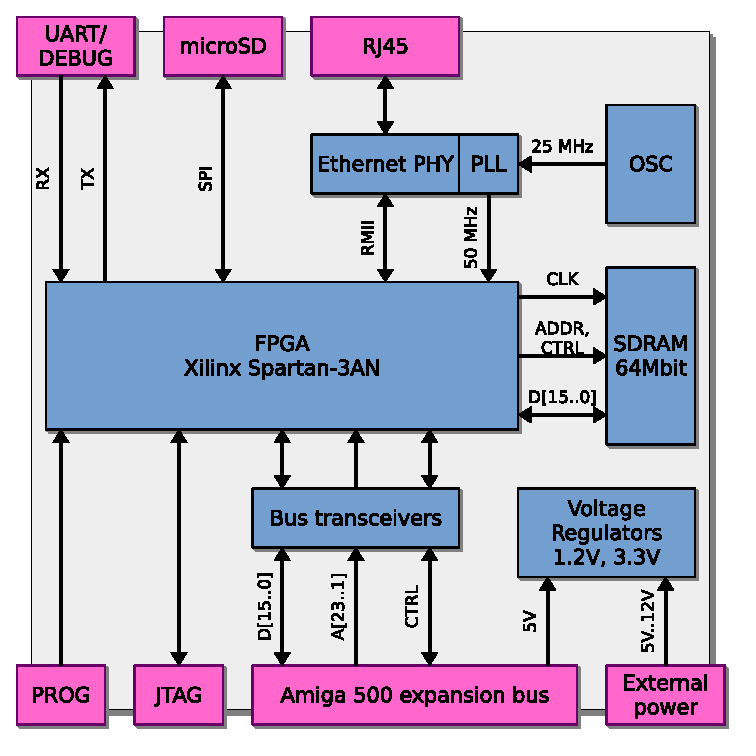
\includegraphics{hw_overview.eps}
\caption{Hardware block diagram of the GRETA expansion
board. Blue boxes indicate on-board devices. Pink boxes are
external connectors.}
\label{hw_overview}
\end{figure}

Figure \ref{hw_overview} illustrates the hardware components
constituting the GRETA expansion board.  For more details,
appendix \ref{greta_sch} contains the electronic schematics
the GRETA expansion board. The schematic files are also the
hardware documentation. Everything needed to reproduce the
hardware is included.

The PCB itself is routed on four layers with the following
stack-up from top to bottom: Signal, ground, 3.3V, signal.
Great care has been taken to achieve good signal integrity
properties. For example, no bus signals or fast switching
signals are routed through vias. Routing is tight; only two
pins on the FPGA are unconnected.

All components, except for external connectors, are surface
mounted. 0603 package is chosen for all resistors and most
capacitors.

Figure \ref{mounted_components2} shows the PCB
with components mounted and figure \ref{greta_connected2} the
expansion board connected to the host computer. Figures
\ref{greta_osh_top} and \ref{greta_osh_bottom} are images rendered
from the Gerber files supplied to the PCB manufacturer.

\begin{figure}
\centering
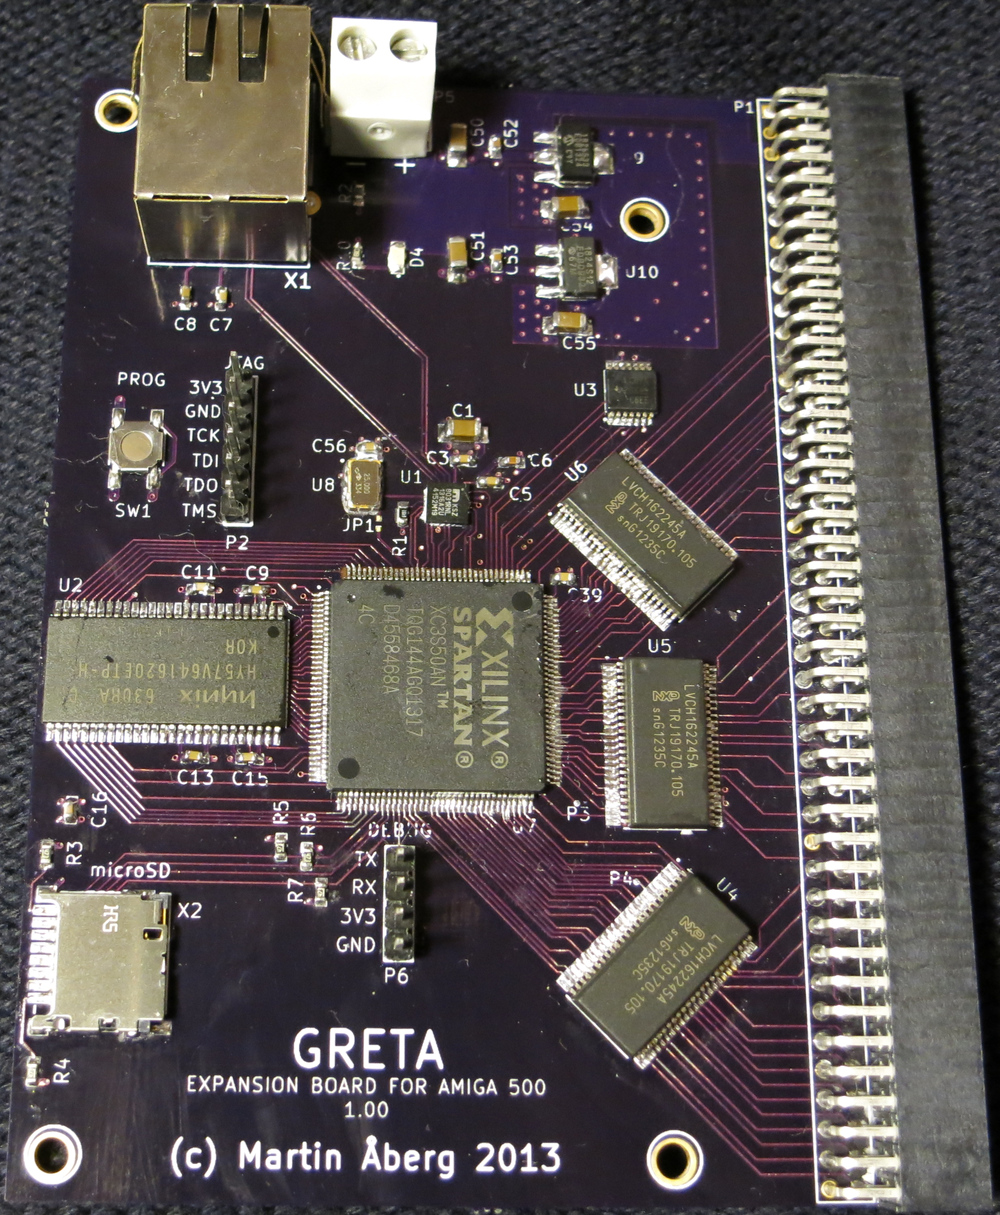
\includegraphics[width=\textwidth]{mounted_components2.jpg}
\caption[LoF entry]{Top side of GRETA expansion board. On the
right edge is the connector to the Amiga computer expansion
bus. The expansion connector has all its signals connected to
three 16-bit transceivers and a 6-bit open drain driver.

Down to the left is the microSD card slot and above it the
SDRAM. At top left is the RJ45 Ethernet connector and next to
it the connector for external power.

The large chip in the middle is the Xilinx FPGA. Above it are
clock oscillator and Ethernet PHY.

Between the expansion connector and external power are two
voltage regulators which generate 1.2V and 3.3V.}
\label{mounted_components2}
\end{figure}

\begin{figure}
\centering
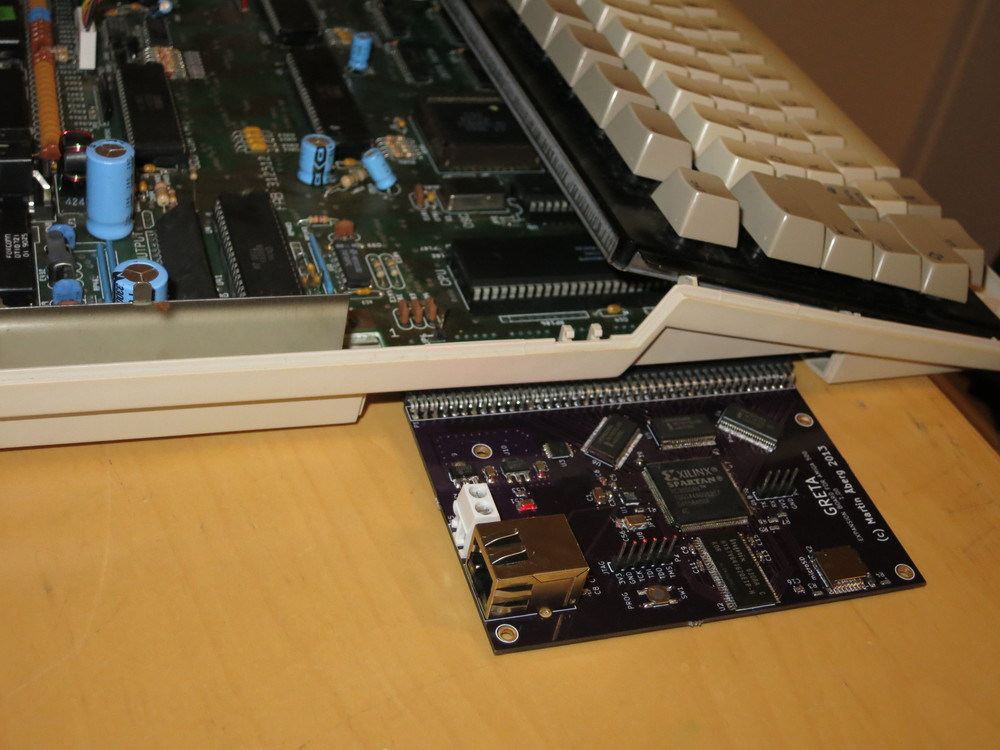
\includegraphics[width=\textwidth]{greta_connected2.jpg}
\caption{The expansion board connects on the left side of the
computer. The large chip parallel to the expansion is the Motorola
MC68000 CPU.}
\label{greta_connected2}
\end{figure}

\begin{figure}
\centering
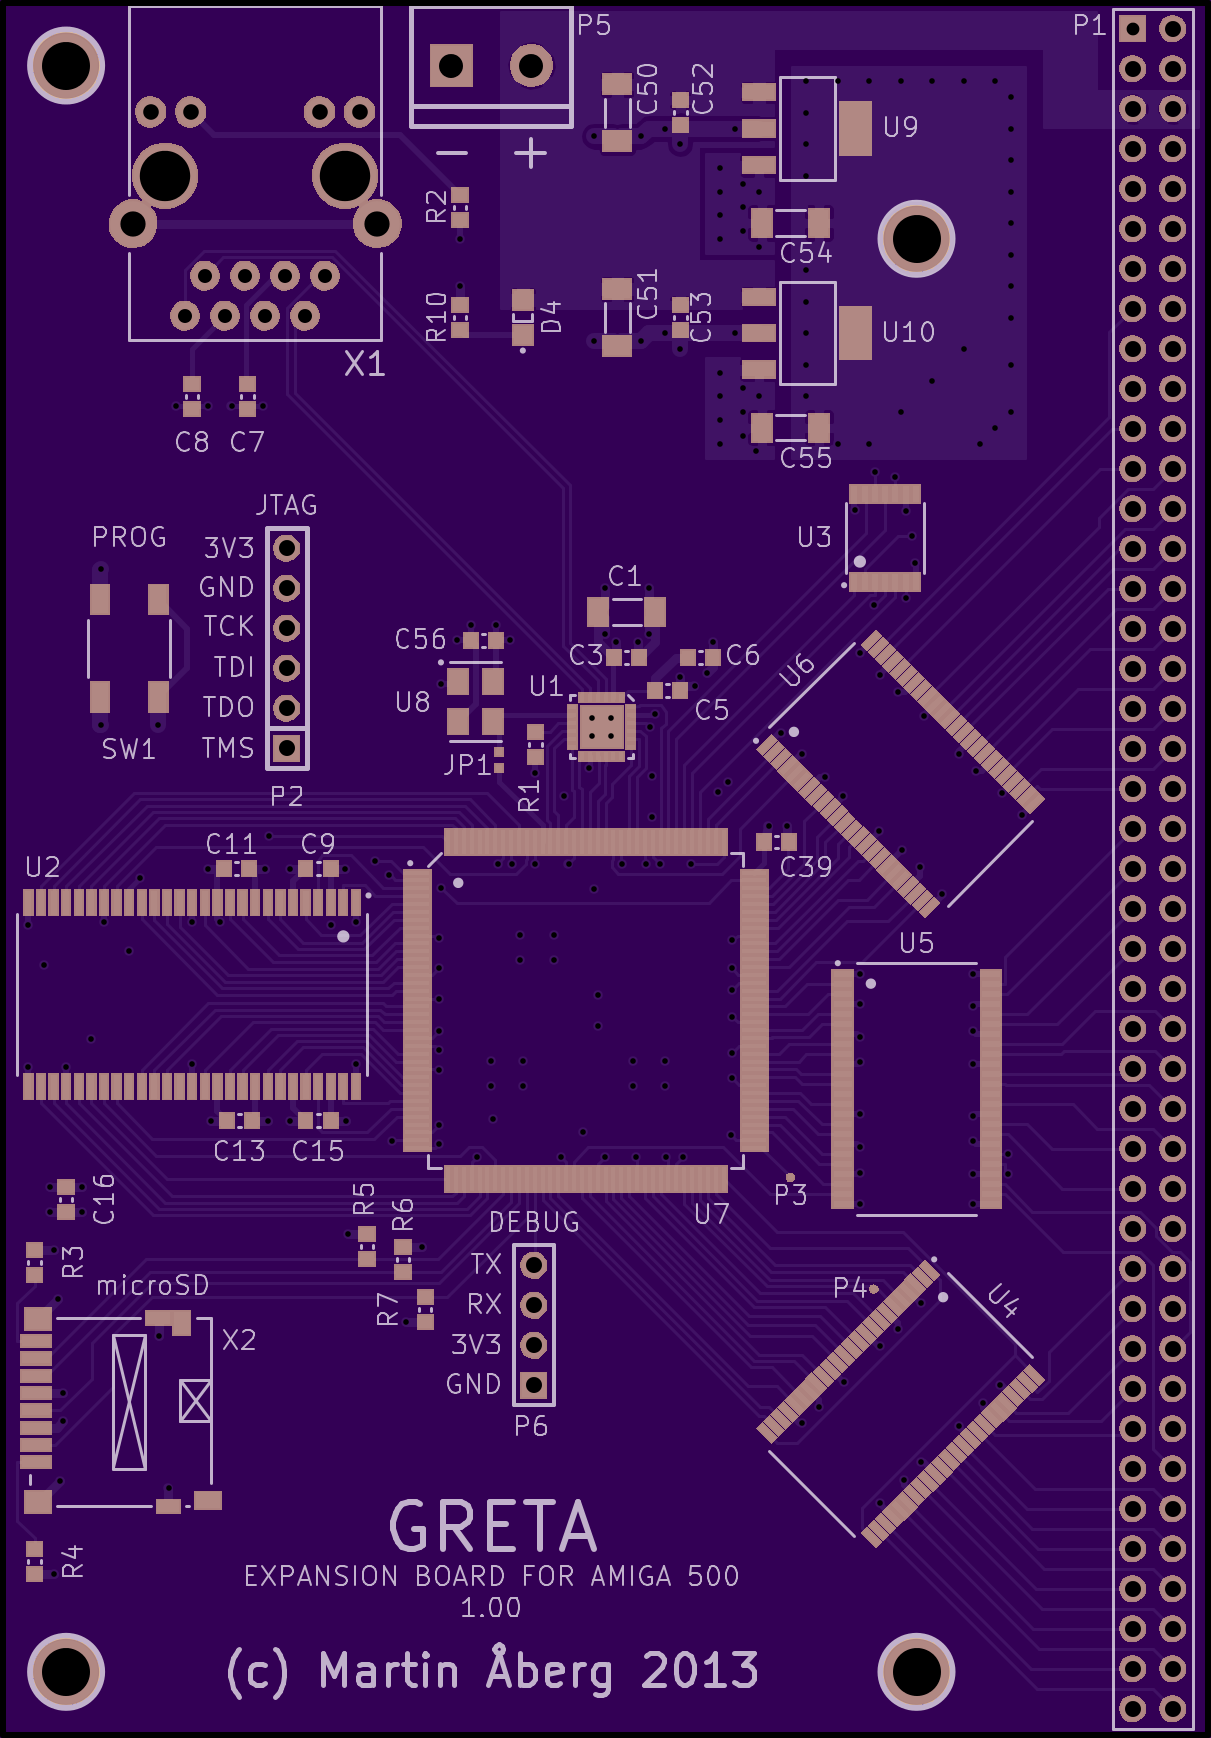
\includegraphics[width=\textwidth]{greta_1_00_top.png}
\caption{PCB top.}
\label{greta_osh_top}
\end{figure}

\begin{figure}
\centering
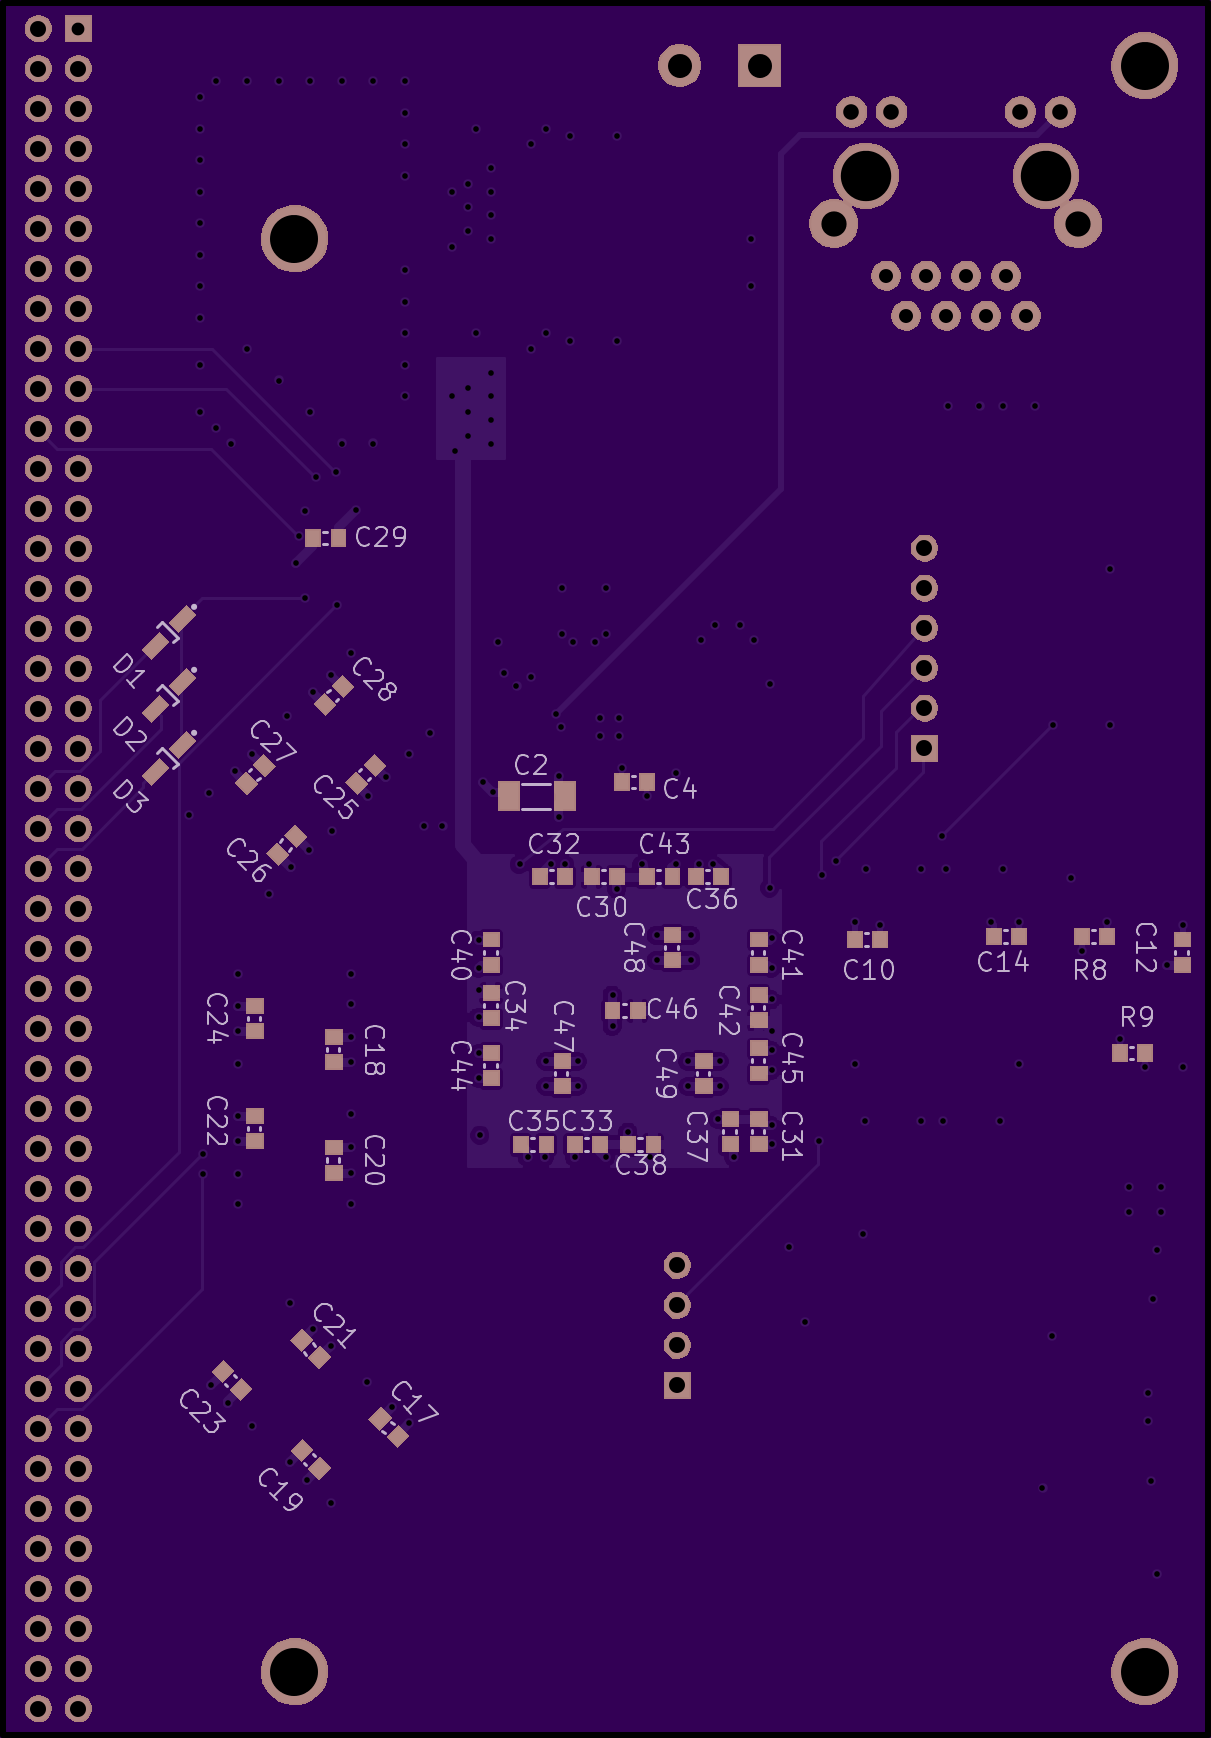
\includegraphics[width=\textwidth]{greta_1_00_bottom.png}
\caption{PCB bottom.}
\label{greta_osh_bottom}
\end{figure}
\subsection{Notes on the hardware design}
The Amiga computer uses 5V TTL signals througout while the FPGA
and the other GRETA components are rated at 3.3V and thus some
signal level conversion is needed. The solution is to use 5V
tolerant drivers for bidirectional signals and unidirectional
signals from the computer to the expansion board. A 16-bit
bidirectional transceiver, NXP 74LVCH162245A, a component with
built-in 30 ohm series termination resistors, solves this. For
signals going from the FPGA back to the computer, the device
SN74LVC07A is used. It has TTL level tolerant open-drain outputs
which fits well with the open collector inputs on the Amiga.

RMII is chosen over MII as Media Independen Interface for the
Ethernet PHY. This reduces pin-count. As a bonus, the selected
chip has a PLL that can feed the FPGA with a clock signal.

\section{Tools}
The following software tools have been used in the development
of the GRETA hardware and HDL.
\begin{description}
  \item[Arch Linux] \hfill \\
  Operating system, tools and infrastructure.
  \item[KiCad, build (2013-may-18)-stable] \hfill \\
  Schematic capture and PCB layout.
  \item[GNU Make] \hfill \\
  Dependecy tracking for compiling documentation and HDL code.
  \item[GHDL 0.30dev (20100112)] \hfill \\
  Functional simulation of HDL code.
  \item[Xilinx ISE 14.6] \hfill \\
  Development environment for Xilinx FPGA.
  \item[ASM-One V1.20] \hfill \\
  Macro-assembler and development environment for the Amiga computer.
  \item[Git] \hfill \\
  Revision control.
  \item[LibreOffice Draw] \hfill \\
  Vector graphics.
  \item[VIM] \hfill \\
  Text editing.
  \item[\LaTeX] \hfill \\
  Typesetting text documents.
\end{description}

\chapter{HDL Overview}
This chapter gives an overview of the GRETA HDL architecture.
All VHDL source files are included in appendix \ref{hdl_code}.
During the devolopment of the HDL components, a set of test
benches were developed. These test benches are not included
in the listings in this document. They are however provided
in the GRETA file distribution.

The top-level module is contained in \texttt{greta.vhdl}
with the port definition described in table \ref{top_level}.
The VHDL package in file \texttt{greta\_pkg.vhdl} contains
type definitions, address constants, bit constants and helper
functions for the other HDL modules. Even though several custom
types are used in the design, the top level ports only use
types defined in \texttt{IEEE.STD\_LOGIC\_1164}.

Figure \ref{hdl_overview} illustrates how the HDL
components are related to each other.

\begin{figure}
\centering
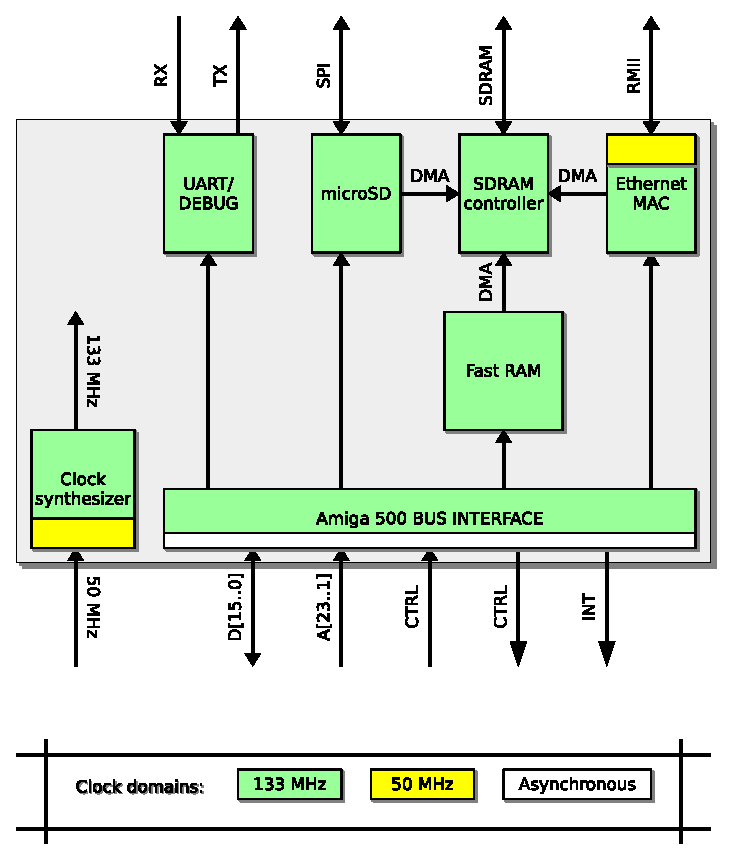
\includegraphics{hdl_overview.eps}
\caption{HDL block diagram of GRETA. Each box represents one
HDL component. All components are implemented using VHDL and
are realised in FPGA.}
\label{hdl_overview}
\end{figure}

\begin{table}
\begin{tabular}{*3l}    \toprule
\emph{Port}             & \emph{Direction}  & \emph{Description} \\ \midrule
\texttt{CLK25MHZ}       & in  & If \texttt{JP1} is open then this input is undefined. \\
\midrule
\midrule
                            &     & Amiga 500 expansion bus\\
\midrule
\texttt{RL\_nRST}           & in  & Reset\\
\texttt{RL\_nAS}            & in  & Address Strobe\\
\texttt{RL\_nUDS}           & in  & Data Upper Strobe\\
\texttt{RL\_nLDS}           & in  & Data Lower Strobe\\
\texttt{RL\_RnW}            & in  & Read/Write\\
\texttt{RL\_CDAC}           & in  & Amiga system clock with 90$^{\circ}$ phase offset\\
\texttt{RL\_nOVR}           & out & Override internal generation of \texttt{nDTACK}\\
\texttt{RL\_nINT2}          & out & Amiga interrupt level 2\\
\texttt{RL\_nINT6}          & out & Amiga interrupt level 6\\
\texttt{RL\_nINT7}          & out & Non-maskable interrupt\\
\texttt{RL\_nDTACK}         & out & Data Acknowledge\\
\texttt{RL\_A[23:1]}        & in  & Address bus \\
\texttt{RL\_D[15:0]}        & inout & Bidirectinal data bus \\
\texttt{RL\_D\_nOE}         & out & Output enable for data bus transceiver \\
\texttt{RL\_D\_TO\_GRETA}   & out & Direction of data bus transceiver\\
\midrule
\midrule
                            &       & SDRAM interface \\
\midrule
\texttt{SDRAM\_CLK}         & out   & Clock \\
\texttt{SDRAM\_CKE}         & out   & Clock Enable \\
\texttt{SDRAM\_nRAS}        & out   & Row Address Strobe \\
\texttt{SDRAM\_nCAS}        & out   & Column Address Strobe \\
\texttt{SDRAM\_nWE}         & out   & Write Enable \\
\texttt{SDRAM\_UDQM}        & out   & Upper Data Input/Output Mask \\
\texttt{SDRAM\_LDQM}        & out   & Lower Data Input/Ouput Mask \\
\texttt{SDRAM\_BA[1:0]}     & out   & Bank Address \\
\texttt{SDRAM\_A[11:0]}     & out   & Address \\
\texttt{SDRAM\_DQ[15:0]}    & inout & Data bus \\
\midrule
\midrule
                    &       & microSD interface (SPI) \\
\midrule
\texttt{SPI\_CLK}   & out   & Clock (SCLK) \\
\texttt{SPI\_nCS}   & out   & Chip Select (SS) \\
\texttt{SPI\_DO}    & out   & Data Output (MOSI) \\
\texttt{SPI\_DI}    & in    & Data Input (MISO)\\
\midrule
\midrule
                        &       & Ethernet PHY (RMII) \\
\midrule
\texttt{PHY\_nRST}      & out   & Reset \\
\texttt{PHY\_MDC}       & out   & MDIO Clock \\
\texttt{PHY\_MDIO}      & inout & MDIO Data I/O \\
\texttt{RMII\_REF\_CLK} & in    & RMII Clock (50 MHz) \\
\texttt{RMII\_CRS\_DV}  & in    & RMII Carrier Sense/Data Valid \\
\texttt{RMII\_RXD[1:0]} & in    & RMII Receive Data \\
\texttt{RMII\_TXD[1:0]} & out   & RMII Transmit Data \\
\texttt{RMII\_TX\_EN}   & out   & RMII Transmit Data Enable \\
\midrule
\midrule
                    &       & UART/DEBUG interface \\
\midrule
\texttt{DEBUG\_RX}  & in    & \\
\texttt{DEBUG\_TX}  & out   & \\
\midrule
\bottomrule
 \hline
\end{tabular}
\caption{GRETA top level ports.}
\label{top_level}
\end{table}

A clock synthesizer unit (DCM) in the FPGA is used to generate
the 133 MHz clock which is used in the internal logic. It is
commonly referred to as the \texttt{clk} signal.

\section{AUTOCONFIG}
According to the AUTOCONFIG protocol of the Amiga computer
ZORRO II specification \cite{a500_techref}, a peripheral
device can be in one of the states \texttt{UNCONFIGURED},
\texttt{CONFIGURED} or \texttt{SHUT\_UP}. After reset,
every device is \texttt{UNCONFIGURED} and responds to bus
accesses in the address space \texttt{\$E80000-\$E8FFFF}
if its \texttt{nCONFIG\_IN} signal is asserted. The system
software reads certain registers from the device in this
area and eventually issues a write to relocate the device
to another address space, typically somewhere inside
\texttt{\$E90000-\$EFFFFF} or \texttt{\$200000-\$9FFFFF}
depending on size requirements. The device is now
\texttt{CONFIGURED} and passes its \texttt{nCONFIG\_OUT} signal
to the next device's \texttt{nCONFIG\_IN}. This procedure is
repeated until all devices in the system are configured.

If the system for some reason choses not to configure a device,
the device is forced into the \texttt{SHUT\_UP} state by writing
to a dedicated register. In this state the device just passes
on its \texttt{nCONFIG\_OUT} and must never respond again
until the next reset.

The AUTOCONFIG space is the address area from
\texttt{\$E80000-\$EFFFFF}. Inside this area there are eight
equaly sized slots.

Definitions and helper functions for the AUTOCONFIG protocol
can be found in the VHDL package \texttt{autoconfig\_pkg}.

\chapter{Bus interface}
The bus decoder is responsible for decoding asynchronous
MC68000 bus signals and exporting a synchronous read/write
protocol to the GRETA peripherals.

\section{Specification}
The internal bus protocl is presented in table
\ref{bus_interface}.

A pulse on \texttt{req} means that \texttt{nwe}, \texttt{addr}
and \texttt{wdata} are valid and will remain so for at least
34 \texttt{clk} periods\footnote{To be decided. This is a
safe minimum.}.

Each GRETA peripheral device holds its \texttt{rdata}
output valid as long as the peripheral is addressed, and zero
otherwise. This allows for all GRETA peripherals to have their
rdata outputs OR-wired to the bus interface \texttt{rdata}
input. An addressed GRETA peripheral must respond to a read
request in 34 \texttt{clk} periods\footnote{To be decided. This
is a safe minimum.} by asserting its \texttt{dev\_select}
signal. The individual \texttt{dev\_select} signals
are OR:ed together at the top level. The bus interface
\texttt{dev\_selected} is used to determine if the bus
transceivers shall drive data towards the Amiga.

The Amiga ZORRO II expansion bus protocol also defines the
signal \texttt{XRDY} which can be used to delay individual
bus accesses. \texttt{XRDY} is not used in the GRETA design
and is not even connected to the GRETA hardware.

\begin{table}
\begin{tabular}{*4l}    \toprule
\emph{Port} & \emph{Type}  & \emph{Direction}  & \emph{Description} \\ \midrule
\texttt{clk}        & \texttt{std\_logic}& in  & GRETA clock\\
\texttt{cpu\_reset} & \texttt{std\_logic}& out & Synchronous reset, activated by Amiga. \\
\midrule
\midrule
                    &                   &       & Internal bus interface \\
\midrule
\texttt{req}        & \texttt{std\_logic}& out & Pulsed once for each 68000 read/write \\
\texttt{nwe}        & \texttt{bus\_nwe} & out  & Upper and lower byte select for write.\\
                    &                   &      & "11" means read. \\
\texttt{addr}       & \texttt{bus\_addr}& out  & Word destination for read and write transfers \\ 
\texttt{wdata}      & \texttt{bus\_data}& out  & WRITE data \\
\texttt{rdata}      & \texttt{bus\_data}& in   & READ data \\
\midrule
\bottomrule
 \hline
\end{tabular}
\caption{Bus interface, internal interface ports.}
\label{bus_interface}
\end{table}

\section{Implementation}
All input signals from the Amiga expansion bus are synchronized
before use in the GRETA clock domain. Control signals have two
synchronizer stages. Stability of sampled data and address
bus signals are assured by the control signals according to
the MC68000 bus protocol. Furthermore, all inputs and outputs
have their registers in the FPGA IO pads.

\chapter{SDRAM Controller}
The SDRAM controller offers a user interface to a physical
SDRAM chip.  Design goals are to provide determinism and an
easy to use control interface.  Performance demands are set
by client access requirements.

All timings in this chapter referes to a \emph{Hynix} SDRAM
chip clocked at 133 MHz and CAS latency of three.

\section{Time resource estimations for SDRAM clients}
The access time requirements for each SDRAM client presented
in the previous chapter are presented in this section and
summarised in Table \ref{sdram_clients}.

\begin{table}
\begin{tabular}{*4l}    \toprule
\emph{Client} & \emph{Period} & \emph{Execution time} & \emph{Deadline} \\
\midrule
Fast RAM      & 55    & 8 & 34   \\
Disk          & 85    & 8 & 85   \\
MAC TX        & 213   & 8 & 213  \\
MAC RX        & 213   & 8 & 213  \\
Auto refresh  & 2083  & 9 & 2083 \\
\bottomrule
 \hline
\end{tabular}
\caption{Real time requirements for clients issuing DMA
operations on SDRAM.  All time values are in units of 133 MHz
clock periods, 7.5ns.  Read and write execution times are based on single 16
bit word access with CAS latency of 3 cycles. Auto refresh is 9 cycles
for this configuration.}
\label{sdram_clients}
\end{table}

\subsection{Fast RAM Controller}
For the ZORRO II bus interface on an NTSC Amiga 500,
accesses can be performed at most once every fourth 7.16MHz
clock cycle \cite{mc68000um}.  The bus read period and
deadlines are derived from \cite{mc68000um} and actual signal
measurements.

Deadline for a bus read is limited by the time at which Motorola
68000 bus samples read data (falling edge leading to bus cycle
state S7).  For bus write, the deadline is effectively the time
at which a following of bus read may occur.  Requests from
bus read and bus write can never be active at the same time
so they are combined to one task in Table \ref{sdram_clients}
to simplify calculations. As a consequence of this, timing
budget for the bus interface is a bit pessimistic.

\subsection{Disk Controller}
A bitrate of 25Mbit/s for Secure Digital over SPI gives a
maximum throughput of 2.98MiB/s. The number of 7.5ns periods
per 16bit SDRAM access is
$85 \le \frac{16 bit}{25 Mbit/s}\cdot \frac{1}{7.5 ns}$.

\subsection{Ethernet MAC}
Periods and deadlines for MAC RX and MAC TX are based on
\si{10}{Mbit} Ethernet in full-duplex mode. With the presented
timing guarantees, only a very narrow FIFO buffer is required
to transfer data between the Ethernet PHY clock domain and
SDRAM. 

The SDRAM access period time for a sustained transfer in each
direction, expressed as 7.5ns periods, is
$213 \le \frac{16 bit}{10 Mbit/s}\cdot \frac{1}{7.5 ns}$.

If support for two word bursts is added to the SDRAM
controller, then \si{100}{Mbit} full-duplex can be supported
without affecting the real time properties of the other RAM
clients. (Though this is possible in theory, the Amiga 500 running
a TCP/IP stack with SANA-II driver interface would never handle
rates above \si{10}{Mbit} anyway.)

\subsection{Auto refresh}
The SDRAM requires 64 refresh operation every 4096 ms. In terms
of 7.5ns periods, this is
$2083 \le \frac{64 ms}{4096}\cdot \frac{1}{7.5 ns}$.

\section{SDRAM Scheduling}
To solve the SDRAM scheduling problem, a static off-line
approach is used. A time table is pre-calculated, in which
each client has its dedicated time slot. An offset pointer
iterates over the calendar slots. When the pointer has reached
the end of the table it restarts from the top again.

This satisfies the goal of determinism and simplicity. Of
course, it must be assured that each client will meet its deadline.

To simplify matters, the accessed bank is always precharged
after an access. Furthermore, if a client does not issue a
request in its designated time slot, the SDRAM will carry out
an unused read operation anyway.  Note that self refreshes
are scheduled just as an ordinary client.

Also note that scheduling of requests to the SDRAM
resource as presented in this section, will result in accesses
not being served in the same time order as they were requested.
Because of this, any of the peripherals must send its interrupt
back to the computer only after an access has been acknowledged
by the RAM arbiter.  Anyhow, requests made by the same client
will always be served in the same order as they were issued.

Table \ref{calendar} illustrates the client calendar. The
tightest timing budget is for a \emph{Disk} request
arriving at time 10 and finishes at time 89, resulting in a
response time of 79 time units.

\begin{table}
\begin{tabular}{*3l}    \toprule
\emph{Offset} & \emph{Time}   & \emph{Client} \\
\midrule
0         &  0 -  8     & Fast RAM      \\
1         &  9 - 17     & Disk          \\
2         & 18 - 26     & Fast RAM      \\
3         & 27 - 35     & MAC TX        \\
4         & 36 - 44     & Fast RAM      \\
5         & 45 - 53     & MAC RX        \\
6         & 54 - 62     & Fast RAM      \\
7         & 63 - 71     & Auto refresh  \\
\midrule            
0         & 72 - 80     & Fast RAM      \\
1         & 81 - 89     & Disk          \\
$\vdots$  & $\vdots$    & $\vdots$      \\
\bottomrule
 \hline
\end{tabular}
\caption{Calendar for static scheduling of the SDRAM resource.
The unit of time offset is one period of a 133 MHz clock (7.5ns).
Calendar has eight positions and repeats after offset 7.}
\label{calendar}
\end{table}

\section{Specification}
Each client communicates with the SDRAM controller
using an in/out signal pair with types \texttt{ram\_bus}
and \texttt{std\_logic} respectively. An example is the
\texttt{fast}/\texttt{fast\_ack} pair. All clients share the
read data bus \texttt{rdata}. See table \ref{ram_bus_type}
for a description of the \texttt{ram\_bus} record type.

Transfers are 16 bit wide but for write accesses, it is
possible to select target bytes individually with the mask
signal \texttt{nwe}.

\begin{table}
\begin{tabular}{*3l}    \toprule
\emph{Member}   & \texttt{Type}         & \emph{Description} \\ \midrule
\texttt{req}    & \texttt{std\_logic}   & Assert high to issue an SDRAM request. \\
\texttt{nwe}    & \texttt{bus\_nwe}     & Upper and lower byte select for write.\\
                &                       & \texttt{"11"} means read. \\
\texttt{addr}   & \texttt{bus\_addr}    & Target address for request. \\
\texttt{wdata}  & \texttt{bus\_data}    & Write data. \\
\bottomrule
 \hline
\end{tabular}
\caption{Record type definition for \texttt{ram\_bus.} The type
is used by SDRAM clients.}
\label{ram_bus_type}
\end{table}

To do an SDRAM request, the client sets its \texttt{req} signal
high and holds it high until the corresponding \texttt{ack}
signal goes high (pulse). The record members \texttt{nwe},
\texttt{addr} and \texttt{wdata} must be constant for the
duration of asserted \texttt{req}.  If it was a read request,
then \texttt{rdata} is valid only in the same clock cycle as
\texttt{ack} is pulsed.

Table \ref{sdram_interface} illustrates the internal HDL
interface to the SDRAM controller.

\begin{table}
\begin{tabular}{*4l}    \toprule
\emph{Port}         & \texttt{Type}         & \emph{Direction}  & \emph{Description} \\ \midrule
\texttt{clk}        & \texttt{std\_logic}   & in  & GRETA clock \\
\texttt{reset}      & \texttt{std\_logic}   & in  & Synchronous reset \\
\midrule
\texttt{ready}      & \texttt{std\_logic}   & out & Controller is ready for requests \\
\midrule
\midrule
                    &                   &       & Fast RAM client \\
\midrule
\texttt{fast}       & \texttt{ram\_bus}     & in  & Control structure for accesses by Disk \\
\texttt{fast\_ack}  & \texttt{std\_logic}   & out & Acknowledge signal for Disk  \\
\midrule
\midrule
                    &                   &       & microSD client \\
\midrule
\texttt{disk}       & \texttt{ram\_bus}     & in  & Control structure for accesses by Disk \\
\texttt{disk\_ack}  & \texttt{std\_logic}   & out & Acknowledge signal for Disk  \\
\midrule
\midrule
                    &                   &       & Ethernet MAC client \\
\midrule
\texttt{mactx}      & \texttt{ram\_bus}     & in  & Control structure for accesses by MAC TX \\
\texttt{mactx\_ack} & \texttt{std\_logic}   & out & Acknowledge signal for MAC TX \\
\midrule
\texttt{macrx}      & \texttt{ram\_bus}     & in  & Control structure for accesses by MAC RX \\
\texttt{macrx\_ack} & \texttt{std\_logic}   & out & Acknowledge signal for MAC RX \\
\midrule
\midrule
                    &                   &       & Common read data bus \\
\midrule
\texttt{rdata}      & \texttt{bus\_data}    & out & Read data, only valid at the corresponding \texttt{\_ack=1} \\ 
\midrule
\bottomrule
 \hline
\end{tabular}
\caption{SDRAM component, interface for internal ports.}
\label{sdram_interface}
\end{table}

\chapter{Fast RAM Controller}
The Fast RAM controller is responsible for implementing the AUTOCONFIG protol
for configuring RAM at system start and then responds to Fast RAM accesses
in the Amiga address range \texttt{\$200000-\$9FFFFF}.

This Amiga address range needs 23 bits to describe 16-bit word
locations. This is a \si{16}{MiB} range but only \si{8}{MiB}
in this range is used for accessing actual RAM. An important
observation is that bit 23 is not significant for addressing
to the SDRAM.

In fact, bit 23 can be ignored. This can be seen by splitting the
Fast RAM address range into three parts and observe the mappings on SDRAM (table \ref{fast_ranges}.

\begin{table}
\begin{tabular}{*3l}    \toprule
\emph{Amiga address}   & \texttt{SDRAM address}         & \texttt{Size} \\ \midrule
\texttt{\$200000-\$3FFFFF} (bit 23=0)& \texttt{\$200000-\$9FFFFF} & \si{2}{MiB}\\
\texttt{\$400000-\$7FFFFF} (bit 23=0)& \texttt{\$400000-\$7FFFFF} & \si{4}{MiB}\\
\texttt{\$800000-\$9FFFFF} (bit 23=1)& \texttt{\$000000-\$1FFFFF} & \si{2}{MiB}\\
\bottomrule
 \hline
\end{tabular}
\caption{Mapping of the external RAM in the Amiga address space to
SDRAM address space.}
\label{fast_ranges}
\end{table}

\section{Specification}
The HDL port interface of the Fast RAM component consists of
the bus interface and the SDRAM interface as described above.


\chapter{Disk Controller}
\section{Specification}
\subsection{User registers}
\section{Implementation}

\appendix
\chapter{Electronic schematics}
\label{greta_sch} 
\begin{centering}
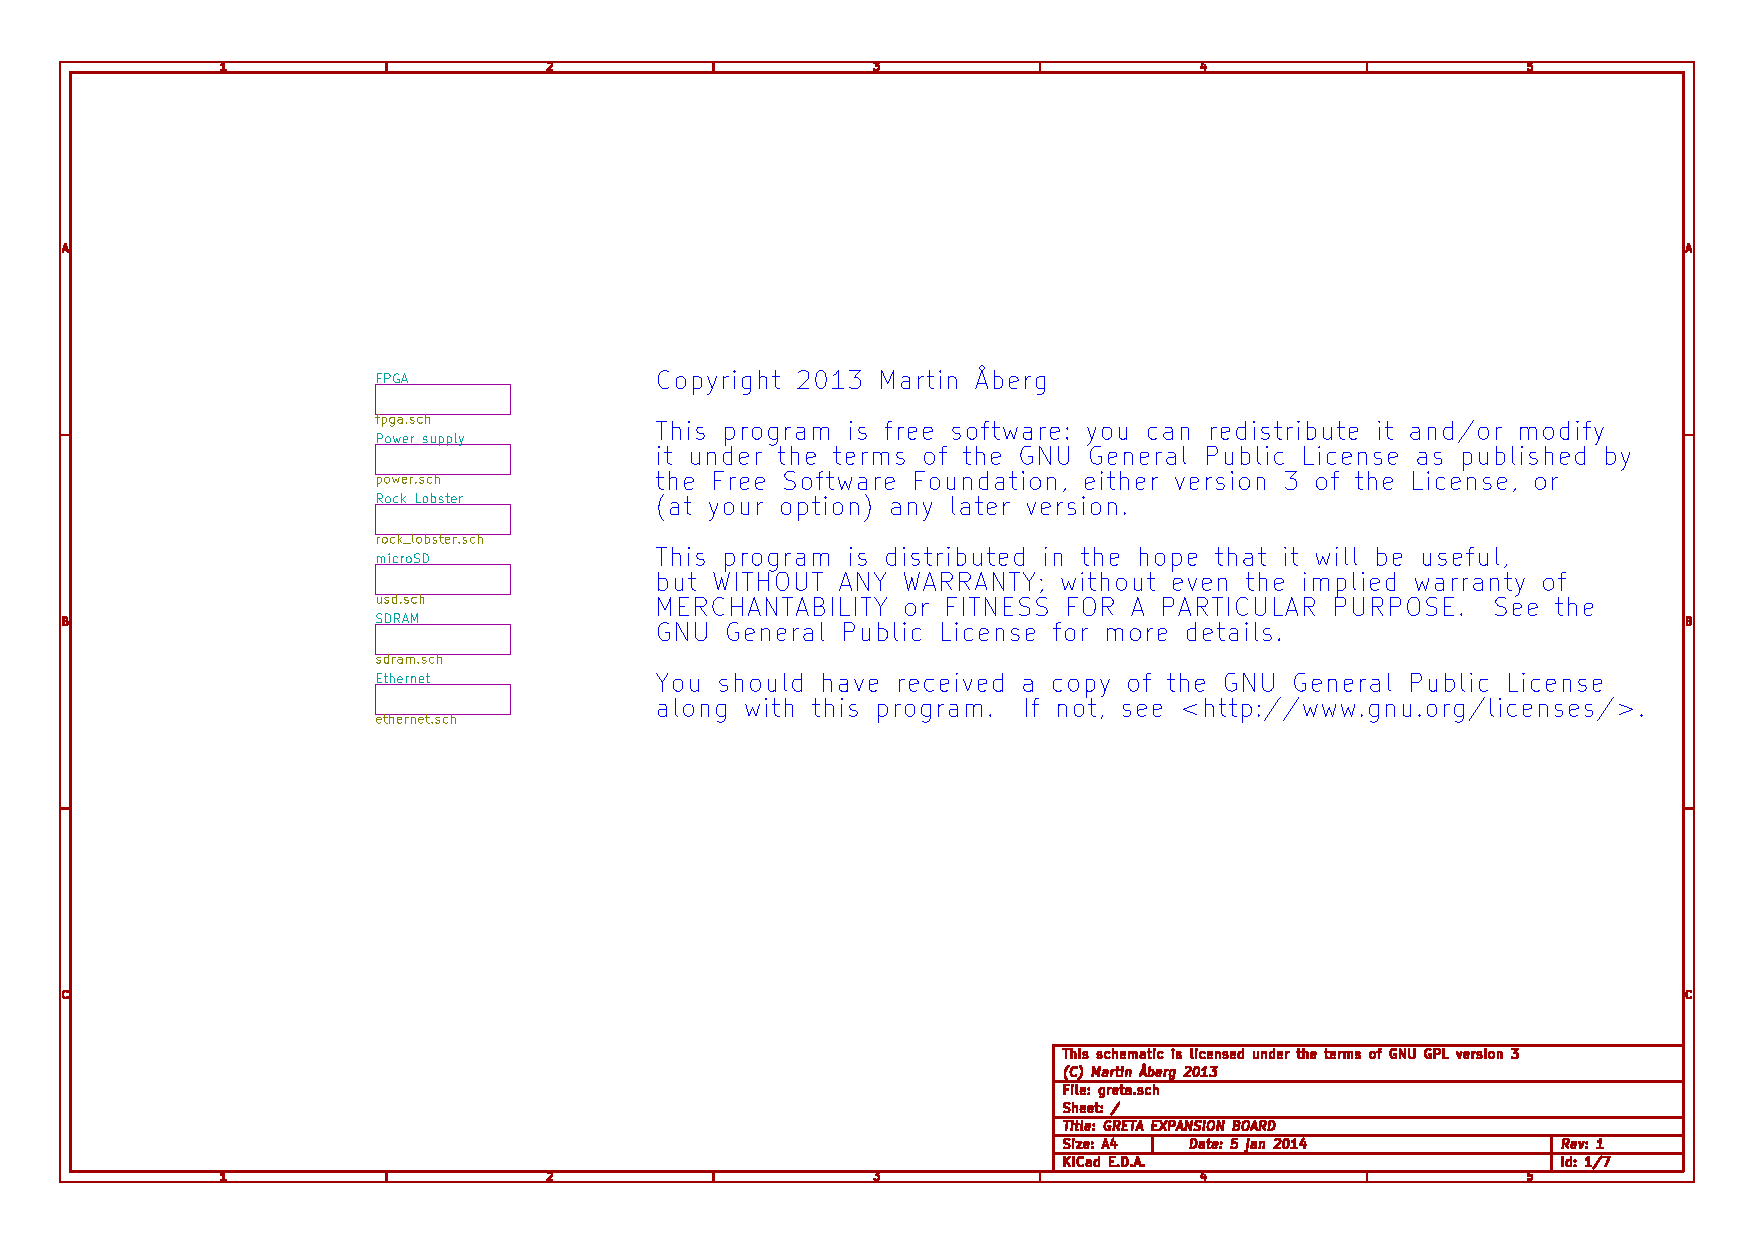
\includegraphics[width=\textwidth, page=1]{schematic.pdf}

\includegraphics[width=\textwidth, page=6]{schematic.pdf}

\includegraphics[width=\textwidth, page=5]{schematic.pdf}

\includegraphics[width=\textwidth, page=3]{schematic.pdf}

\includegraphics[width=\textwidth, page=2]{schematic.pdf}

\includegraphics[width=\textwidth, page=4]{schematic.pdf}

\includegraphics[width=\textwidth, page=7]{schematic.pdf}
\end{centering}

\chapter{HDL code}
\label{hdl_code}

\section{GRETA types, constants and functions}
    \lstinputlisting{../hdl/greta_pkg.vhdl}

\newpage
\section{GRETA}
    \lstinputlisting{../hdl/greta.vhdl}

\newpage
\section{Bus Interface}
    \lstinputlisting{../hdl/bus_interface/bus_interface.vhdl}

\newpage
\section{SDRAM Controller}
    \lstinputlisting{../hdl/sdram/sdram.vhdl}

\newpage
\section{Fast RAM Controller}
    \lstinputlisting{../hdl/fast/fast.vhdl}

\newpage
\section{Disk Controller}
    \lstinputlisting{../hdl/disk/disk.vhdl}


\chapter{GNU Free Documentation License}
\phantomsection  % so hyperref creates bookmarks
\addcontentsline{toc}{chapter}{GNU Free Documentation License}
%\label{label_fdl}

 \begin{center}

       Version 1.3, 3 November 2008


 Copyright \copyright{} 2000, 2001, 2002, 2007, 2008  Free Software Foundation, Inc.
 
 \bigskip
 
     \texttt{<http://fsf.org/>}
  
 \bigskip
 
 Everyone is permitted to copy and distribute verbatim copies
 of this license document, but changing it is not allowed.
\end{center}


\begin{center}
{\bf\large Preamble}
\end{center}

The purpose of this License is to make a manual, textbook, or other
functional and useful document ``free'' in the sense of freedom: to
assure everyone the effective freedom to copy and redistribute it,
with or without modifying it, either commercially or noncommercially.
Secondarily, this License preserves for the author and publisher a way
to get credit for their work, while not being considered responsible
for modifications made by others.

This License is a kind of ``copyleft'', which means that derivative
works of the document must themselves be free in the same sense.  It
complements the GNU General Public License, which is a copyleft
license designed for free software.

We have designed this License in order to use it for manuals for free
software, because free software needs free documentation: a free
program should come with manuals providing the same freedoms that the
software does.  But this License is not limited to software manuals;
it can be used for any textual work, regardless of subject matter or
whether it is published as a printed book.  We recommend this License
principally for works whose purpose is instruction or reference.


\begin{center}
{\Large\bf 1. APPLICABILITY AND DEFINITIONS\par}
\phantomsection
\addcontentsline{toc}{section}{1. APPLICABILITY AND DEFINITIONS}
\end{center}

This License applies to any manual or other work, in any medium, that
contains a notice placed by the copyright holder saying it can be
distributed under the terms of this License.  Such a notice grants a
world-wide, royalty-free license, unlimited in duration, to use that
work under the conditions stated herein.  The ``\textbf{Document}'', below,
refers to any such manual or work.  Any member of the public is a
licensee, and is addressed as ``\textbf{you}''.  You accept the license if you
copy, modify or distribute the work in a way requiring permission
under copyright law.

A ``\textbf{Modified Version}'' of the Document means any work containing the
Document or a portion of it, either copied verbatim, or with
modifications and/or translated into another language.

A ``\textbf{Secondary Section}'' is a named appendix or a front-matter section of
the Document that deals exclusively with the relationship of the
publishers or authors of the Document to the Document's overall subject
(or to related matters) and contains nothing that could fall directly
within that overall subject.  (Thus, if the Document is in part a
textbook of mathematics, a Secondary Section may not explain any
mathematics.)  The relationship could be a matter of historical
connection with the subject or with related matters, or of legal,
commercial, philosophical, ethical or political position regarding
them.

The ``\textbf{Invariant Sections}'' are certain Secondary Sections whose titles
are designated, as being those of Invariant Sections, in the notice
that says that the Document is released under this License.  If a
section does not fit the above definition of Secondary then it is not
allowed to be designated as Invariant.  The Document may contain zero
Invariant Sections.  If the Document does not identify any Invariant
Sections then there are none.

The ``\textbf{Cover Texts}'' are certain short passages of text that are listed,
as Front-Cover Texts or Back-Cover Texts, in the notice that says that
the Document is released under this License.  A Front-Cover Text may
be at most 5 words, and a Back-Cover Text may be at most 25 words.

A ``\textbf{Transparent}'' copy of the Document means a machine-readable copy,
represented in a format whose specification is available to the
general public, that is suitable for revising the document
straightforwardly with generic text editors or (for images composed of
pixels) generic paint programs or (for drawings) some widely available
drawing editor, and that is suitable for input to text formatters or
for automatic translation to a variety of formats suitable for input
to text formatters.  A copy made in an otherwise Transparent file
format whose markup, or absence of markup, has been arranged to thwart
or discourage subsequent modification by readers is not Transparent.
An image format is not Transparent if used for any substantial amount
of text.  A copy that is not ``Transparent'' is called ``\textbf{Opaque}''.

Examples of suitable formats for Transparent copies include plain
ASCII without markup, Texinfo input format, LaTeX input format, SGML
or XML using a publicly available DTD, and standard-conforming simple
HTML, PostScript or PDF designed for human modification.  Examples of
transparent image formats include PNG, XCF and JPG.  Opaque formats
include proprietary formats that can be read and edited only by
proprietary word processors, SGML or XML for which the DTD and/or
processing tools are not generally available, and the
machine-generated HTML, PostScript or PDF produced by some word
processors for output purposes only.

The ``\textbf{Title Page}'' means, for a printed book, the title page itself,
plus such following pages as are needed to hold, legibly, the material
this License requires to appear in the title page.  For works in
formats which do not have any title page as such, ``Title Page'' means
the text near the most prominent appearance of the work's title,
preceding the beginning of the body of the text.

The ``\textbf{publisher}'' means any person or entity that distributes
copies of the Document to the public.

A section ``\textbf{Entitled XYZ}'' means a named subunit of the Document whose
title either is precisely XYZ or contains XYZ in parentheses following
text that translates XYZ in another language.  (Here XYZ stands for a
specific section name mentioned below, such as ``\textbf{Acknowledgements}'',
``\textbf{Dedications}'', ``\textbf{Endorsements}'', or ``\textbf{History}''.)  
To ``\textbf{Preserve the Title}''
of such a section when you modify the Document means that it remains a
section ``Entitled XYZ'' according to this definition.

The Document may include Warranty Disclaimers next to the notice which
states that this License applies to the Document.  These Warranty
Disclaimers are considered to be included by reference in this
License, but only as regards disclaiming warranties: any other
implication that these Warranty Disclaimers may have is void and has
no effect on the meaning of this License.


\begin{center}
{\Large\bf 2. VERBATIM COPYING\par}
\phantomsection
\addcontentsline{toc}{section}{2. VERBATIM COPYING}
\end{center}

You may copy and distribute the Document in any medium, either
commercially or noncommercially, provided that this License, the
copyright notices, and the license notice saying this License applies
to the Document are reproduced in all copies, and that you add no other
conditions whatsoever to those of this License.  You may not use
technical measures to obstruct or control the reading or further
copying of the copies you make or distribute.  However, you may accept
compensation in exchange for copies.  If you distribute a large enough
number of copies you must also follow the conditions in section~3.

You may also lend copies, under the same conditions stated above, and
you may publicly display copies.


\begin{center}
{\Large\bf 3. COPYING IN QUANTITY\par}
\phantomsection
\addcontentsline{toc}{section}{3. COPYING IN QUANTITY}
\end{center}


If you publish printed copies (or copies in media that commonly have
printed covers) of the Document, numbering more than 100, and the
Document's license notice requires Cover Texts, you must enclose the
copies in covers that carry, clearly and legibly, all these Cover
Texts: Front-Cover Texts on the front cover, and Back-Cover Texts on
the back cover.  Both covers must also clearly and legibly identify
you as the publisher of these copies.  The front cover must present
the full title with all words of the title equally prominent and
visible.  You may add other material on the covers in addition.
Copying with changes limited to the covers, as long as they preserve
the title of the Document and satisfy these conditions, can be treated
as verbatim copying in other respects.

If the required texts for either cover are too voluminous to fit
legibly, you should put the first ones listed (as many as fit
reasonably) on the actual cover, and continue the rest onto adjacent
pages.

If you publish or distribute Opaque copies of the Document numbering
more than 100, you must either include a machine-readable Transparent
copy along with each Opaque copy, or state in or with each Opaque copy
a computer-network location from which the general network-using
public has access to download using public-standard network protocols
a complete Transparent copy of the Document, free of added material.
If you use the latter option, you must take reasonably prudent steps,
when you begin distribution of Opaque copies in quantity, to ensure
that this Transparent copy will remain thus accessible at the stated
location until at least one year after the last time you distribute an
Opaque copy (directly or through your agents or retailers) of that
edition to the public.

It is requested, but not required, that you contact the authors of the
Document well before redistributing any large number of copies, to give
them a chance to provide you with an updated version of the Document.


\begin{center}
{\Large\bf 4. MODIFICATIONS\par}
\phantomsection
\addcontentsline{toc}{section}{4. MODIFICATIONS}
\end{center}

You may copy and distribute a Modified Version of the Document under
the conditions of sections 2 and 3 above, provided that you release
the Modified Version under precisely this License, with the Modified
Version filling the role of the Document, thus licensing distribution
and modification of the Modified Version to whoever possesses a copy
of it.  In addition, you must do these things in the Modified Version:

\begin{itemize}
\item[A.] 
   Use in the Title Page (and on the covers, if any) a title distinct
   from that of the Document, and from those of previous versions
   (which should, if there were any, be listed in the History section
   of the Document).  You may use the same title as a previous version
   if the original publisher of that version gives permission.
   
\item[B.]
   List on the Title Page, as authors, one or more persons or entities
   responsible for authorship of the modifications in the Modified
   Version, together with at least five of the principal authors of the
   Document (all of its principal authors, if it has fewer than five),
   unless they release you from this requirement.
   
\item[C.]
   State on the Title page the name of the publisher of the
   Modified Version, as the publisher.
   
\item[D.]
   Preserve all the copyright notices of the Document.
   
\item[E.]
   Add an appropriate copyright notice for your modifications
   adjacent to the other copyright notices.
   
\item[F.]
   Include, immediately after the copyright notices, a license notice
   giving the public permission to use the Modified Version under the
   terms of this License, in the form shown in the Addendum below.
   
\item[G.]
   Preserve in that license notice the full lists of Invariant Sections
   and required Cover Texts given in the Document's license notice.
   
\item[H.]
   Include an unaltered copy of this License.
   
\item[I.]
   Preserve the section Entitled ``History'', Preserve its Title, and add
   to it an item stating at least the title, year, new authors, and
   publisher of the Modified Version as given on the Title Page.  If
   there is no section Entitled ``History'' in the Document, create one
   stating the title, year, authors, and publisher of the Document as
   given on its Title Page, then add an item describing the Modified
   Version as stated in the previous sentence.
   
\item[J.]
   Preserve the network location, if any, given in the Document for
   public access to a Transparent copy of the Document, and likewise
   the network locations given in the Document for previous versions
   it was based on.  These may be placed in the ``History'' section.
   You may omit a network location for a work that was published at
   least four years before the Document itself, or if the original
   publisher of the version it refers to gives permission.
   
\item[K.]
   For any section Entitled ``Acknowledgements'' or ``Dedications'',
   Preserve the Title of the section, and preserve in the section all
   the substance and tone of each of the contributor acknowledgements
   and/or dedications given therein.
   
\item[L.]
   Preserve all the Invariant Sections of the Document,
   unaltered in their text and in their titles.  Section numbers
   or the equivalent are not considered part of the section titles.
   
\item[M.]
   Delete any section Entitled ``Endorsements''.  Such a section
   may not be included in the Modified Version.
   
\item[N.]
   Do not retitle any existing section to be Entitled ``Endorsements''
   or to conflict in title with any Invariant Section.
   
\item[O.]
   Preserve any Warranty Disclaimers.
\end{itemize}

If the Modified Version includes new front-matter sections or
appendices that qualify as Secondary Sections and contain no material
copied from the Document, you may at your option designate some or all
of these sections as invariant.  To do this, add their titles to the
list of Invariant Sections in the Modified Version's license notice.
These titles must be distinct from any other section titles.

You may add a section Entitled ``Endorsements'', provided it contains
nothing but endorsements of your Modified Version by various
parties---for example, statements of peer review or that the text has
been approved by an organization as the authoritative definition of a
standard.

You may add a passage of up to five words as a Front-Cover Text, and a
passage of up to 25 words as a Back-Cover Text, to the end of the list
of Cover Texts in the Modified Version.  Only one passage of
Front-Cover Text and one of Back-Cover Text may be added by (or
through arrangements made by) any one entity.  If the Document already
includes a cover text for the same cover, previously added by you or
by arrangement made by the same entity you are acting on behalf of,
you may not add another; but you may replace the old one, on explicit
permission from the previous publisher that added the old one.

The author(s) and publisher(s) of the Document do not by this License
give permission to use their names for publicity for or to assert or
imply endorsement of any Modified Version.


\begin{center}
{\Large\bf 5. COMBINING DOCUMENTS\par}
\phantomsection
\addcontentsline{toc}{section}{5. COMBINING DOCUMENTS}
\end{center}


You may combine the Document with other documents released under this
License, under the terms defined in section~4 above for modified
versions, provided that you include in the combination all of the
Invariant Sections of all of the original documents, unmodified, and
list them all as Invariant Sections of your combined work in its
license notice, and that you preserve all their Warranty Disclaimers.

The combined work need only contain one copy of this License, and
multiple identical Invariant Sections may be replaced with a single
copy.  If there are multiple Invariant Sections with the same name but
different contents, make the title of each such section unique by
adding at the end of it, in parentheses, the name of the original
author or publisher of that section if known, or else a unique number.
Make the same adjustment to the section titles in the list of
Invariant Sections in the license notice of the combined work.

In the combination, you must combine any sections Entitled ``History''
in the various original documents, forming one section Entitled
``History''; likewise combine any sections Entitled ``Acknowledgements'',
and any sections Entitled ``Dedications''.  You must delete all sections
Entitled ``Endorsements''.

\begin{center}
{\Large\bf 6. COLLECTIONS OF DOCUMENTS\par}
\phantomsection
\addcontentsline{toc}{section}{6. COLLECTIONS OF DOCUMENTS}
\end{center}

You may make a collection consisting of the Document and other documents
released under this License, and replace the individual copies of this
License in the various documents with a single copy that is included in
the collection, provided that you follow the rules of this License for
verbatim copying of each of the documents in all other respects.

You may extract a single document from such a collection, and distribute
it individually under this License, provided you insert a copy of this
License into the extracted document, and follow this License in all
other respects regarding verbatim copying of that document.


\begin{center}
{\Large\bf 7. AGGREGATION WITH INDEPENDENT WORKS\par}
\phantomsection
\addcontentsline{toc}{section}{7. AGGREGATION WITH INDEPENDENT WORKS}
\end{center}


A compilation of the Document or its derivatives with other separate
and independent documents or works, in or on a volume of a storage or
distribution medium, is called an ``aggregate'' if the copyright
resulting from the compilation is not used to limit the legal rights
of the compilation's users beyond what the individual works permit.
When the Document is included in an aggregate, this License does not
apply to the other works in the aggregate which are not themselves
derivative works of the Document.

If the Cover Text requirement of section~3 is applicable to these
copies of the Document, then if the Document is less than one half of
the entire aggregate, the Document's Cover Texts may be placed on
covers that bracket the Document within the aggregate, or the
electronic equivalent of covers if the Document is in electronic form.
Otherwise they must appear on printed covers that bracket the whole
aggregate.


\begin{center}
{\Large\bf 8. TRANSLATION\par}
\phantomsection
\addcontentsline{toc}{section}{8. TRANSLATION}
\end{center}


Translation is considered a kind of modification, so you may
distribute translations of the Document under the terms of section~4.
Replacing Invariant Sections with translations requires special
permission from their copyright holders, but you may include
translations of some or all Invariant Sections in addition to the
original versions of these Invariant Sections.  You may include a
translation of this License, and all the license notices in the
Document, and any Warranty Disclaimers, provided that you also include
the original English version of this License and the original versions
of those notices and disclaimers.  In case of a disagreement between
the translation and the original version of this License or a notice
or disclaimer, the original version will prevail.

If a section in the Document is Entitled ``Acknowledgements'',
``Dedications'', or ``History'', the requirement (section~4) to Preserve
its Title (section~1) will typically require changing the actual
title.


\begin{center}
{\Large\bf 9. TERMINATION\par}
\phantomsection
\addcontentsline{toc}{section}{9. TERMINATION}
\end{center}


You may not copy, modify, sublicense, or distribute the Document
except as expressly provided under this License.  Any attempt
otherwise to copy, modify, sublicense, or distribute it is void, and
will automatically terminate your rights under this License.

However, if you cease all violation of this License, then your license
from a particular copyright holder is reinstated (a) provisionally,
unless and until the copyright holder explicitly and finally
terminates your license, and (b) permanently, if the copyright holder
fails to notify you of the violation by some reasonable means prior to
60 days after the cessation.

Moreover, your license from a particular copyright holder is
reinstated permanently if the copyright holder notifies you of the
violation by some reasonable means, this is the first time you have
received notice of violation of this License (for any work) from that
copyright holder, and you cure the violation prior to 30 days after
your receipt of the notice.

Termination of your rights under this section does not terminate the
licenses of parties who have received copies or rights from you under
this License.  If your rights have been terminated and not permanently
reinstated, receipt of a copy of some or all of the same material does
not give you any rights to use it.


\begin{center}
{\Large\bf 10. FUTURE REVISIONS OF THIS LICENSE\par}
\phantomsection
\addcontentsline{toc}{section}{10. FUTURE REVISIONS OF THIS LICENSE}
\end{center}


The Free Software Foundation may publish new, revised versions
of the GNU Free Documentation License from time to time.  Such new
versions will be similar in spirit to the present version, but may
differ in detail to address new problems or concerns.  See
\texttt{http://www.gnu.org/copyleft/}.

Each version of the License is given a distinguishing version number.
If the Document specifies that a particular numbered version of this
License ``or any later version'' applies to it, you have the option of
following the terms and conditions either of that specified version or
of any later version that has been published (not as a draft) by the
Free Software Foundation.  If the Document does not specify a version
number of this License, you may choose any version ever published (not
as a draft) by the Free Software Foundation.  If the Document
specifies that a proxy can decide which future versions of this
License can be used, that proxy's public statement of acceptance of a
version permanently authorizes you to choose that version for the
Document.


\begin{center}
{\Large\bf 11. RELICENSING\par}
\phantomsection
\addcontentsline{toc}{section}{11. RELICENSING}
\end{center}


``Massive Multiauthor Collaboration Site'' (or ``MMC Site'') means any
World Wide Web server that publishes copyrightable works and also
provides prominent facilities for anybody to edit those works.  A
public wiki that anybody can edit is an example of such a server.  A
``Massive Multiauthor Collaboration'' (or ``MMC'') contained in the
site means any set of copyrightable works thus published on the MMC
site.

``CC-BY-SA'' means the Creative Commons Attribution-Share Alike 3.0
license published by Creative Commons Corporation, a not-for-profit
corporation with a principal place of business in San Francisco,
California, as well as future copyleft versions of that license
published by that same organization.

``Incorporate'' means to publish or republish a Document, in whole or
in part, as part of another Document.

An MMC is ``eligible for relicensing'' if it is licensed under this
License, and if all works that were first published under this License
somewhere other than this MMC, and subsequently incorporated in whole
or in part into the MMC, (1) had no cover texts or invariant sections,
and (2) were thus incorporated prior to November 1, 2008.

The operator of an MMC Site may republish an MMC contained in the site
under CC-BY-SA on the same site at any time before August 1, 2009,
provided the MMC is eligible for relicensing.


\begin{center}
{\Large\bf ADDENDUM: How to use this License for your documents\par}
\phantomsection
\addcontentsline{toc}{section}{ADDENDUM: How to use this License for your documents}
\end{center}

To use this License in a document you have written, include a copy of
the License in the document and put the following copyright and
license notices just after the title page:

\bigskip
\begin{quote}
    Copyright \copyright{}  YEAR  YOUR NAME.
    Permission is granted to copy, distribute and/or modify this document
    under the terms of the GNU Free Documentation License, Version 1.3
    or any later version published by the Free Software Foundation;
    with no Invariant Sections, no Front-Cover Texts, and no Back-Cover Texts.
    A copy of the license is included in the section entitled ``GNU
    Free Documentation License''.
\end{quote}
\bigskip
    
If you have Invariant Sections, Front-Cover Texts and Back-Cover Texts,
replace the ``with \dots\ Texts.''\ line with this:

\bigskip
\begin{quote}
    with the Invariant Sections being LIST THEIR TITLES, with the
    Front-Cover Texts being LIST, and with the Back-Cover Texts being LIST.
\end{quote}
\bigskip
    
If you have Invariant Sections without Cover Texts, or some other
combination of the three, merge those two alternatives to suit the
situation.

If your document contains nontrivial examples of program code, we
recommend releasing these examples in parallel under your choice of
free software license, such as the GNU General Public License,
to permit their use in free software.

\begin{thebibliography}{9}

\bibitem{a500_techref}
  Commodore Business Machines,
  \emph{Commodore A500/A2000 Techincal Reference Manual}.
  1986, 1987.

\bibitem{gdbserial}
  Richard Stallman, Roland Pesch, Stan Shebbs, et al, 
  \emph{Debugging with GDB: The GNU Source-Level Debugger}.
  Free Software Foundation,
  10th Edition,
  2014.
  \url{http://www.gnu.org/software/gdb/documentation/}

\bibitem{mc68000um}
  Motorola, Inc,
  \emph{M68000 User's Manual}.
  Prentice-Hall, Inc,
  8th Edition,
  1990.

\end{thebibliography}

\end{document}

